\documentclass{zjureport-zh}

\projtype{本科生课程实验报告}
\projname{OpenMP PI}
\course{并行计算与多核编程}
\name{陈卓}
\stuid{3170101214}
\college{计算机科学与技术}
\major{计算机科学与技术}
\instructor{楼学庆}



\begin{document}

\makecover

\section{介绍}
\par 计算无理数 $\pi$ 的值在数值计算中是一个长久的问题。自 Chunovsky 兄弟将 $\pi$ 计算至 10 亿位后,Chunovsky 算法甚至成为了一种业余地测试计算机性能的方式。本次试验选取一种较为简单的算法和 Chunovsky 算法计算 $\pi$,并用 OpenMP 实现它们的并行算法。完整代码在 \hyperlink{https://github.com/zhuo34/openmp-pi}{GitHub}。

\section{实验平台}
\begin{enumerate}[label=(\arabic*)]
	\item 2.3 GHz 双核Intel Core i5
	\item clang 10.0.0
	\item OpenMP 8.0.0
\end{enumerate}

\section{算法}
\subsection{积分}
\par 我们可以通过简单的定积分来完成 $\pi$ 的计算。
\begin{equation}
	\pi = \int_0^1 \frac{4}{1+x^2} dx \label{eq1}
\end{equation}

\par 由公式 \ref{eq1} 我们可以获取一种计算 $\pi$ 的方法,即将区间 $[0, 1]$ 分为 $N$ 份,通过累加的方式计算这个定积分。
\par 代码如下。
\begin{lstlisting}[language=c++]
std::string pi_simple(int N, int n_threads) {
	mpf_class sum = 0;
	mpf_class step = 1.0 / N;
	mpf_class x;
	for (int i = 0; i < N; i++) {
		x = ( i + 0.5 ) * step;
		sum += 4.0 / (1.0 + x * x);
	}
	mpf_class pi = sum*step;
	mp_exp_t exp;
	return pi.get_str(exp);
}
\end{lstlisting}


\subsection{Chunovsky 算法}
\par 算法一简单易懂,但它的收敛速度自然是很慢的,$N$ 扩大十倍大约能增加 2 位精度。为了提升收敛,众多数学家提出了各种各样的级数,Chunovsky 级数就是其中最有代表性之一。\footnote{因为这次实验侧重点在计算,Chunovsky 级数的证明在此不做叙述。}
\begin{equation}
	\frac{1}{\pi} = 12\cdot\sum\limits_{n=0}^{\infty} \frac{(-1)^n(6n)!}{(3n)!(n!)^3} \cdot \frac{13591409+545140134n}{640320^{3n+3/2}} \label{eq2}
\end{equation}

\par 观察公式 \ref{eq2},其中每一项有大量的乘除法运算,而众所周知,乘除法的效率远比加减法低,因此可以用到 Binary Splitting 技术对计算过程加速。它的核心思想是将每一项的分数合并为加法,最终只进行一次或少量乘除法。\cite{webref}\cite{haible1998fast}

\par 代码如下。
\begin{lstlisting}[language=c++]
void bs(long a, long b, mpz_class &P, mpz_class &Q, mpz_class &T) {
	if (b - a == 1) {
		if (a == 0) {
			P = Q = mpz_class(1);
		} else {
			P = mpz_class((6*a-5)*(2*a-1)*(6*a-1));
			Q = mpz_class(a*a*a*C3_OVER_24);
		}
		T = P * (13591409 + 545140134*a);
		if (a%2 == 1) {
			T = -T;
		}
	} else {
		long m = (a + b) / 2;
		mpz_class Pam, Qam, Tam;
		mpz_class Pmb, Qmb, Tmb;
		bs(a, m, Pam, Qam, Tam);
		bs(m, b, Pmb, Qmb, Tmb);
		P = Pam * Pmb;
		Q = Qam * Qmb;
		T = Qmb * Tam + Pam * Tmb;
	}
}

std::string pi_chudnovsky(unsigned int digits) {
	mpf_set_default_prec(digits*log2(10));
	mpf_class DIGITS_PER_TERM = log(C3_OVER_24.get_d()/6/2/6);
	mpf_class a = digits/DIGITS_PER_TERM + 1;
	long N = a.get_si();
	mpz_class P, Q, T;
	bs(0, N * 10, P, Q, T);
	mpf_class pi = (Q * 426880 * my_sqrt(10005)) / T;
	mp_exp_t exp;
	std::string ret = pi.get_str(exp);
	return ret;
}
\end{lstlisting}


\section{用 OpenMP 实现的并行算法}
\par 对于算法一,我们可以将 OpenMP 运用在循环中,并用 reduction 处理 \texttt{sum} 变量。相关代码如下。
\begin{lstlisting}[language=c++]
std::string pi_simple(int N, int n_threads) {
	...
	#pragma omp parallel for private( x ) reduction(+: sum) num_threads(n_threads)
	for (int i = 0; i < N; i++) {
		x = ( i + 0.5 ) * step;
		sum += 4.0 / (1.0 + x * x);
	}
	...
}
\end{lstlisting}

\par 对于算法二,我们可以将 OpenMP 运用在 \texttt{bs} 函数的递归调用中,因此需要一个变量记录递归深度,如果线程用完则串行执行。相关代码如下。
\begin{lstlisting}[language=c++]
void bs(long a, long b, mpz_class &P, mpz_class &Q, mpz_class &T, int max_depth=0)
{
	...
	if (max_depth > 0) {
	#pragma omp parallel sections default(shared)
	{
	#pragma omp section
		{
			bs(a, m, Pam, Qam, Tam, max_depth - 1);
		}
	#pragma omp section
		{
			bs(m, b, Pmb, Qmb, Tmb, max_depth-1);
		}
	}
	} else {
		bs(a, m, Pam, Qam, Tam, max_depth);
		bs(m, b, Pmb, Qmb, Tmb, max_depth);
	}
	...
}
\end{lstlisting}

\section{测试结果与讨论}
\par 对于算法一,因为它的收敛性达不到要求,因此我们只关注 OpenMP 的加速效果。
\begin{figure}[h]
	\subfigure[耗时]{
		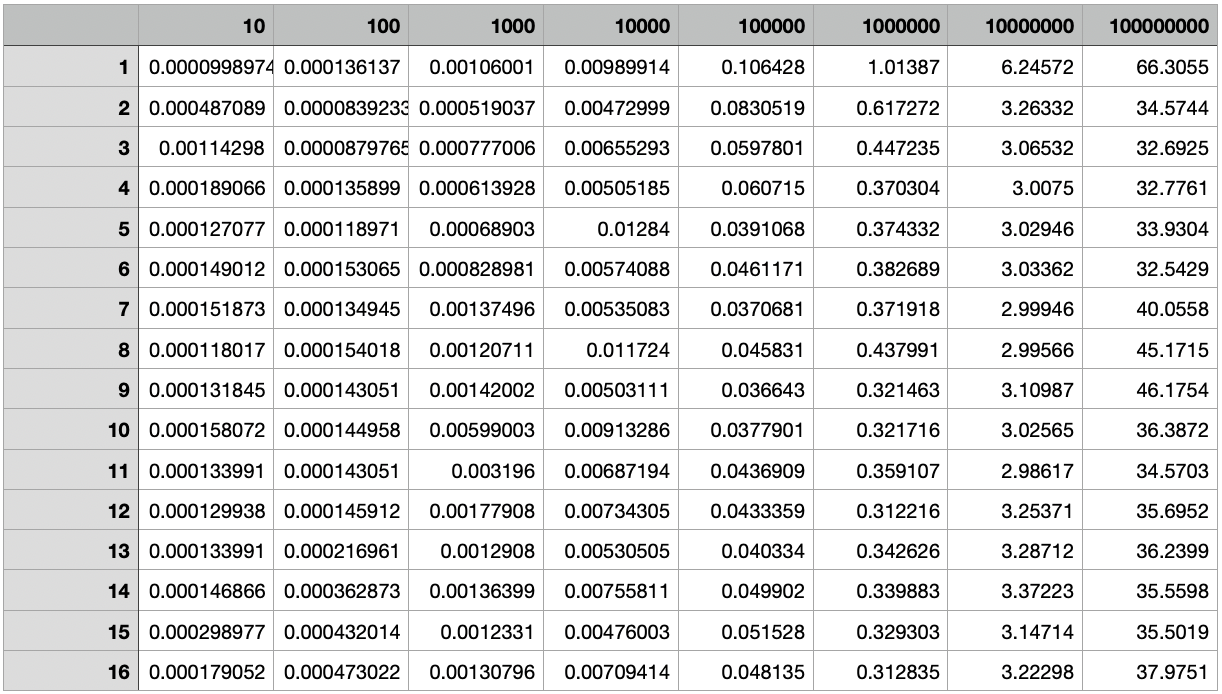
\includegraphics[width=.5\linewidth]{imgs/time_s}
	}
	\subfigure[加速比]{
		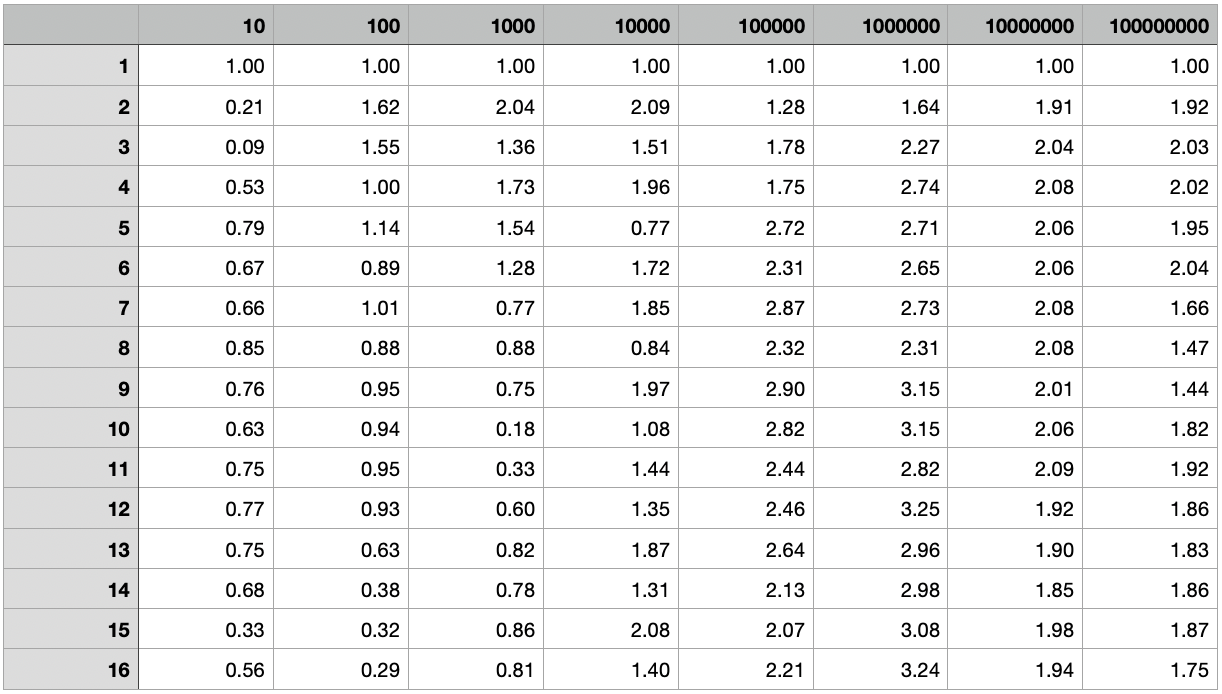
\includegraphics[width=.5\linewidth]{imgs/speed_s}
	}
	\subfigure[耗时数据图]{
		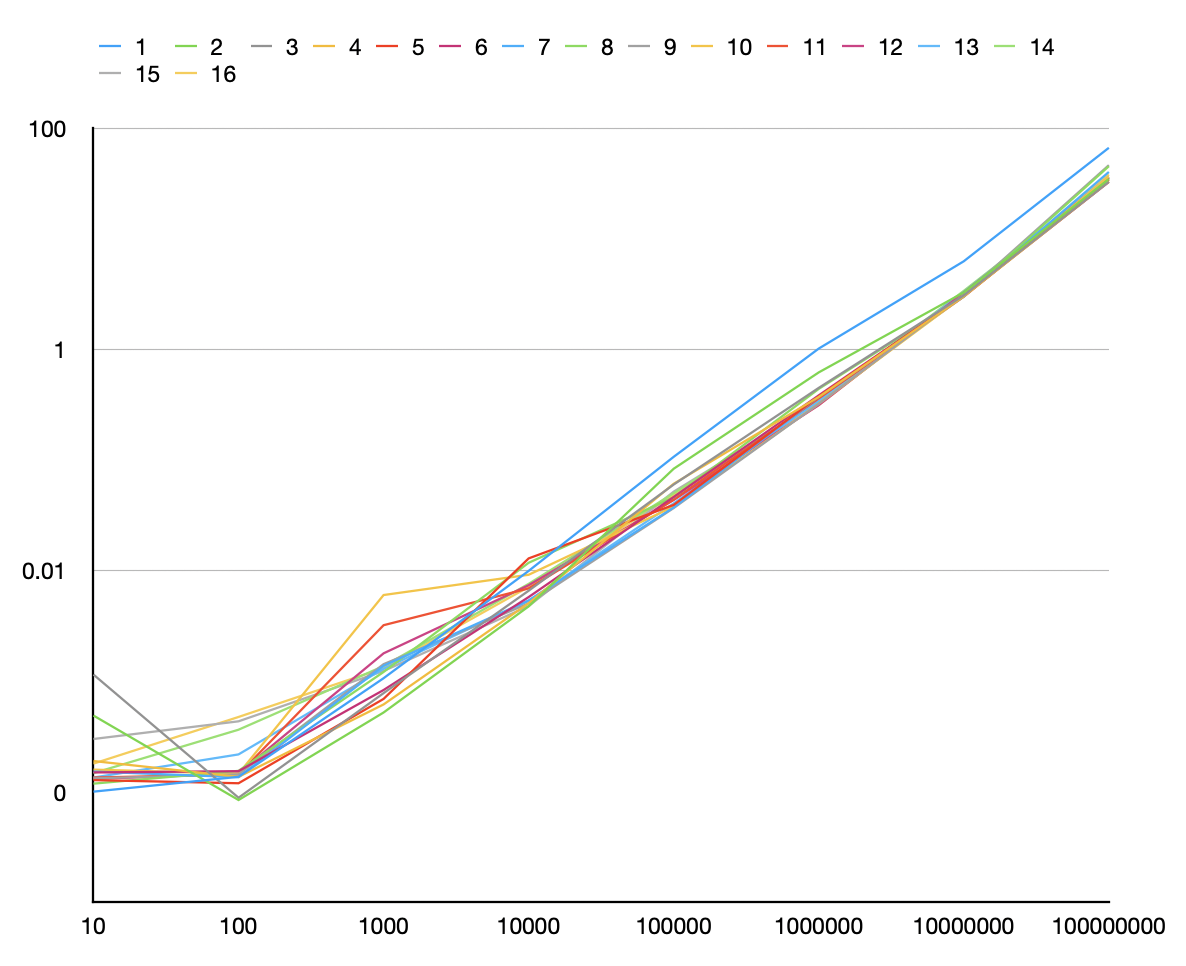
\includegraphics[width=.5\linewidth]{imgs/graph_s0}
	}
	\subfigure[耗时数据图(大数据量部分)]{
		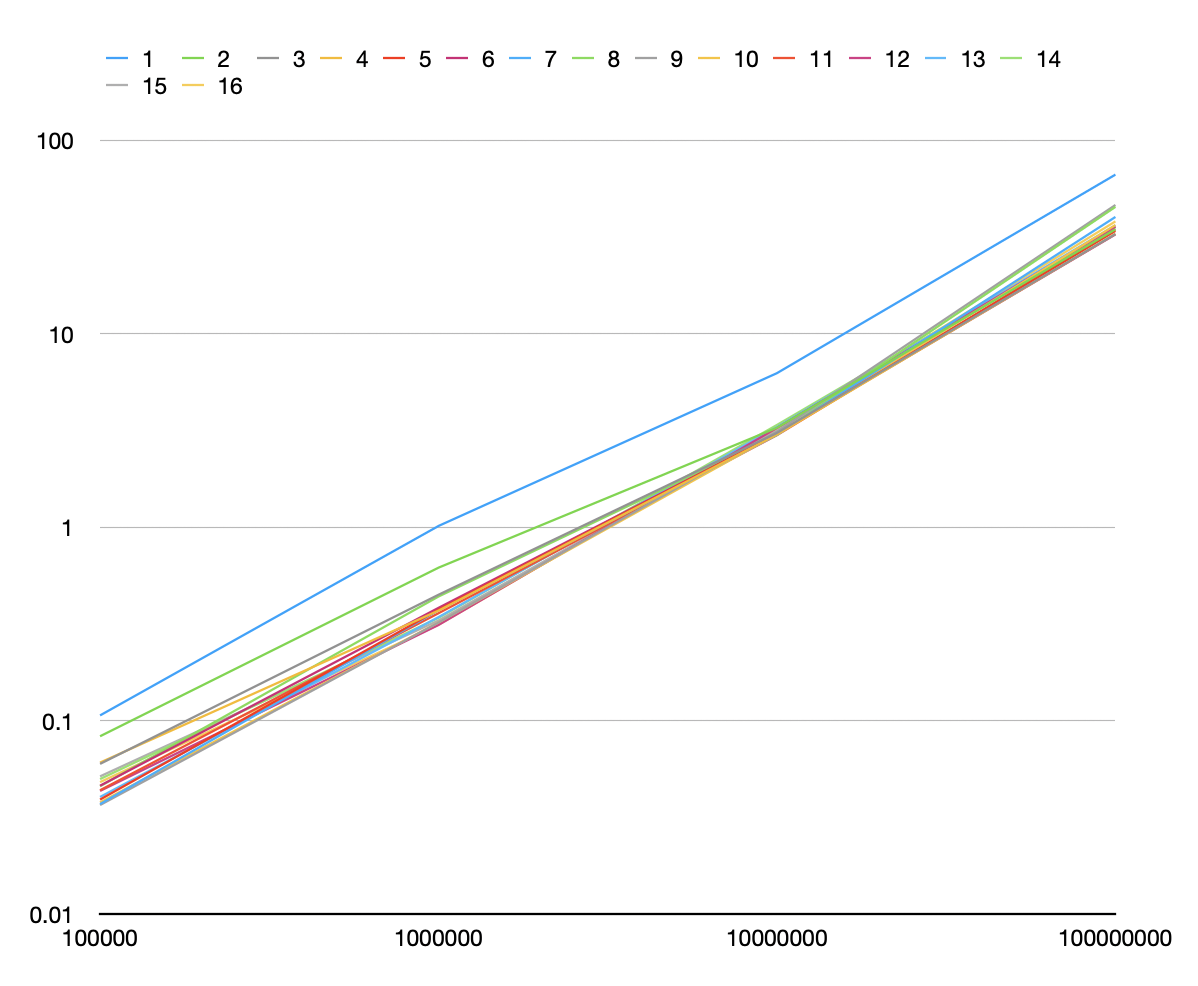
\includegraphics[width=.5\linewidth]{imgs/graph_s1}
	}
	\caption{算法一}
\end{figure}
\par 从图表来看,算法一在 4 线程时表现最好,大约有 2 的加速比。

\par 对于算法二,我们可以从图表数据 \ref{fig2} 中清晰地看出它的线性收敛性\footnote{图中纵轴对数化以保持与测试时计算位数 10 倍增长的一致性。}。并且在 2 线程时效果最好,获得 1.7 左右的加速比。

\begin{figure}[h] \label{fig2}
	\centering
	\subfigure[耗时]{
		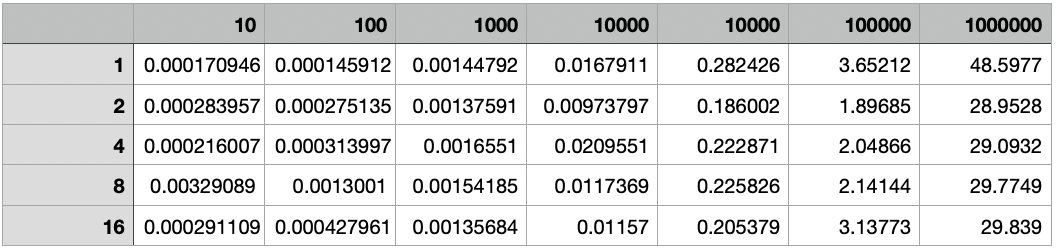
\includegraphics[width=.5\linewidth]{imgs/time_c}
	}\subfigure[加速比]{
		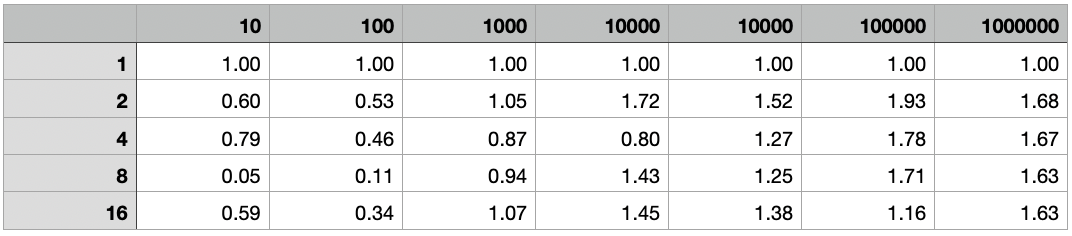
\includegraphics[width=.5\linewidth]{imgs/speed_c}
	}
	\subfigure[耗时数据图]{
		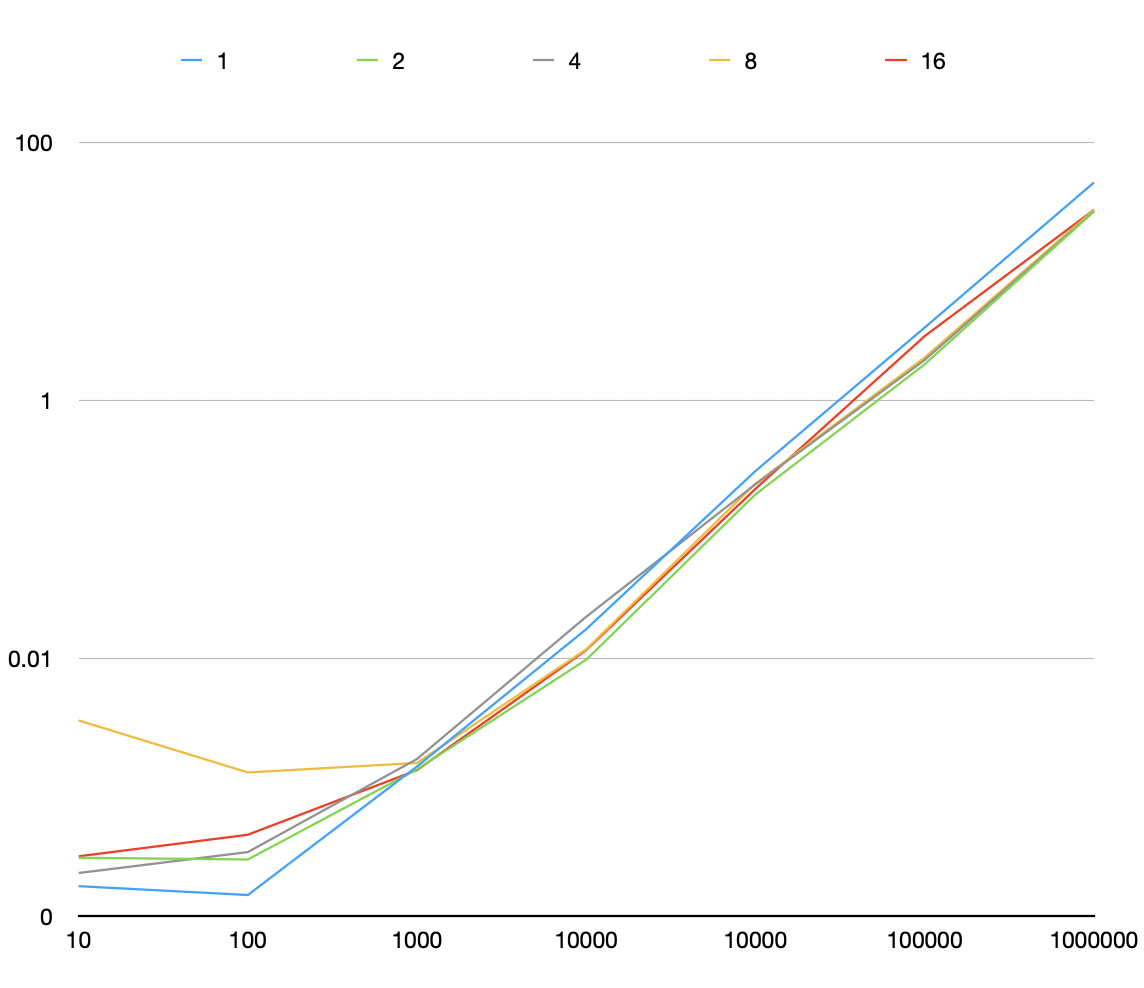
\includegraphics[width=.75\linewidth]{imgs/graph_c}
	}
	\caption{算法二}
\end{figure}

\par 此次试验通过计算 $\pi$ 运用了 OpenMP 并行框架,掌握了 OpenMP/C++ 的并行代码编写能力,体会了其中的并行思想,收获颇丰。

\bibliographystyle{plain}
\bibliography{refs}

\end{document}










